\documentclass{article}
\usepackage{graphics}
\usepackage{graphicx}
\usepackage{tabularx}
\usepackage[titletoc,title]{appendix}

\title{SBS trigger and electronics update}

\author{A. Camsonne, M. K. Jones}

\begin{document}
\maketitle
\section{Experiment overview}

\section{Electronics inventory}

\section{Jefferson Laboratory Infrastructure}
\subsection {Network bandwith}
Infrastructure upgrade was completed.
Connection from Hall A to the Computer Center is done on one 10 GBit giving a maximum bandwidth
of 1.25 GB/s. Hall D was able to have a 700 MB/s sustained rate.
the link is upgradeable to 40 GBit when it will be cost effective to switch to it.
\subsection {Tape silo}
Tape silo is  and is using LTO format. LTO7 was deployed in 2015, each tape in this format
can hold 6.25 TB and transfer data at 300 MB/s natively.
Up to a factor two might be possible with built in compression.
Cost of tape has been steadily coming down.

\begin{tabular}{|c|c|c|c|}
  \hline
  & Data TB & LTO7 \\
  \hline
  &  & &\\
  \hline
\end{tabular}
\section{Electronics for SuperBigbite spectrometer}
\subsection{CODA}
Jefferson Laboratory is using the Cebaf Online Data Acquisition system for data taking.
CODA is based on a main server interacting with a database in which all the DAQ components update their status . The readout crates host a single board computer running a Read Out Controller (ROC) program which controls and reads out the data from the electronics. The ROCs send the data through a standard network link usually ethernet to a computer running the Event Builder program, which uses the data from the ROC to check synchronization and build the event. Finally the event is sent to the Event Recorder which puts the event into a file on the hard drive of the computer. 
\subsection{CODA Hardware}
In addition to the software a set of harware components specific to CODA is used in order to keep ensure event synchronization between all the components each crate has a trigger interface ( TI board ) which sends the trigger signal to the ROC program for the read out of the data. All the TI are linked to a trigger supervisor board which takes the triggers and sends them to the TI while monitoring the status of each TI to keep all the crates synchronized and generates a Level 1 accept and Level 2 accept for the read out modules. The TS also takes as input the front end busy of the modules to inhibit the triggering if one module is not ready insuring synchronization between the modules.
This allows the TS module to buffering if the front-end has the capability. The triggers and read out are then decorrelated which improve the deadtime since a module can take triggers while being readout asynchronously. The TS has a setting of the maximum of events which can be in the buffer it is set to the smallest buffer available on the electronics ( usually 5 for fastbus ). Since in this mode modules can potentially get out of synchronization, a synchronization event is set so that when a certain number of triggers is processed, the TS will disable the triggers to empty the FIFO. If there any remaining events in the FIFO a warning issue would be issued and the FIFOs would be cleared resynchronizing the modules.

\includegraphics[scale=0.55]{figs/TS.pdf}\\

\subsubsection{Trigger Interface}
The Trigger Interface (TI) is a VME board designed to initiate the readout of the modules in the crate. The TI insures 
\subsubsection{Trigger Supervisor}
The Trigger Supervisor takes the trigger in and provides gates to the different modules from the data acquisition system.
It gathers the busy signal from the TI and all the modules and will inhibit the triggers if one module is not ready keeping all the components synchronized for each event. The TS also allows buffering, for a buffer depth set to the minimum buffer depth of the module with the smallest buffer. In our case the 1877S has a buffer depth of 8 events. This allows to 
\subsection{Pipelined electronics}
\subsubsection{JLab Flash ADC 250}


The JLab Flash ADC 250
\subsubsection{F1 TDC}
\subsubsection{SubSystem Processor}
\subsubsection{VXS Trigger Processor}
\subsubsection{Signal Distribution}

\section{GEM readout}
\subsection{APV25}
The GEM readout is carried out by the APV25 chip. It is a 128 channels ASICs with pipeline depth of 192 samples sampling at 40 MHz giving a pipeline depth of 4.8 $\mu s$ ( limited to 4 $\mu s$ for the hardware to perform correctly) . When a trigger is issued the corresponding cells are frozen until they are readout while the other cells are still being used reducing the dead time.
For each trigger all the data of 128 channels are transfered at 40 MHz rate in a multiplexed analog format. Adding some header and event informations 141 words are transmitted for each trigger which gives a transfer time of $141x25 ns = 3.6 \mu s $. In case of high background several consecutives time samples can be sent in order to detect pile up, we plan to read 3 samples which gives a transfer time of 10.8 $\mu s$. If the we assume the controls words are recorded on 32 bits and each sample is recorded on 16 bit this gives a raw event size of (141-128)*4+(128*2)*3 = 820 bytes per APV. This allows deadtimeless operation for rates up to 90 KHz.

\subsection {Multi Purpose Digitizer (MPD)}
 The readout planned to be use the the INFN Multi Purpose Digitizer (MPD), it is a VME board with a 200 MHz FADC and signals to control the APV setup and readout. It has 2 ports which can read up to 8 APVs each for a total of 16 APVs giving 2048 channels. 
For the GEp trackers 14 APVs will be read per MPDs, the APV data is 130 24 bit words so the event size to be transferred for 3 samples is then :

$130 ( words per APV ) * 3 (samples ) * 14 (APV ) * 3 (bytes ) = 16.38 KB $

Several readout schemes are possible with the MPD.  The board could also transfer the data through VXS port or through the optical link. The board complies with the VME64X standard and can transfer up to 200 MB/s in sustained rate using the VME320 protocol on the VME64X backplane. 

\begin{figure}
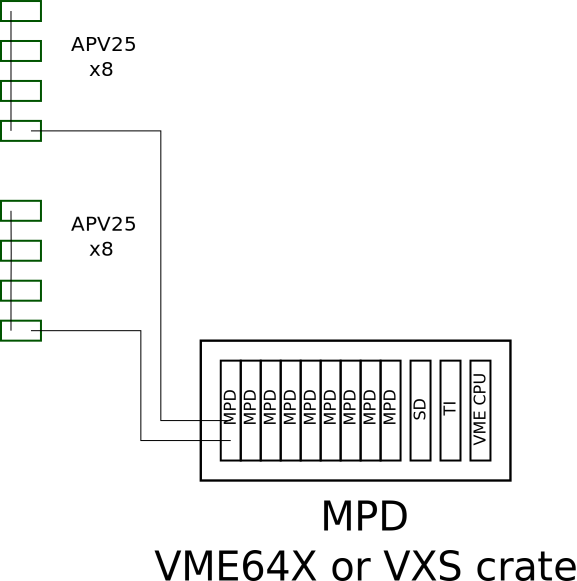
\includegraphics[scale=0.55]{figs/OldMPD.pdf}\\
\end{figure}
Though taking into account overhead of the transaction, we assume we can transfer a sustained rate of about 100 MB/s.

At the assumed maximum rate of 5 KHz ( expected is 3 KHz ), that gives a raw data rate of 81.9 MB/s going into the MPD from the APVs.


In the case of the GEp5, it was estimated that occupancy was around 60\% which would corresponds then to 49.2 MB/s per MPD after zero suppression which would give 2 MPDs per crates. 

To reduce the data the deconvolution algorithm will be implemented on the MPD to improve the timing resolution and reduce the occupancy by effectively shortening the pulse, we expect a factor of 3 reduction of the accidental background.

In order to further reduce the cost and amount of data recorded on tape a new readout scheme was proposed taking advantage of the JLAB electronics and optical link feature of the MPD.

\includegraphics[scale=0.55]{figs/NewMPD.pdf}\\

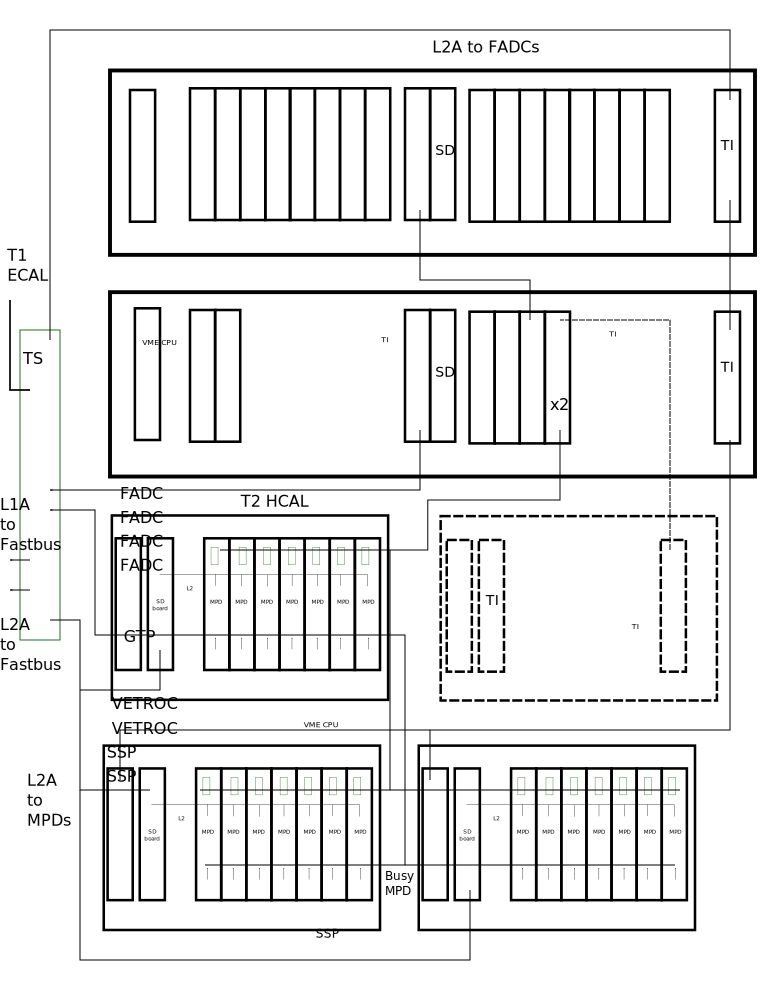
\includegraphics[scale=0.55]{figs/NewMPDDetailed.pdf}\\

\includegraphics[scale=0.55]{figs/MPD4_UserManual.pdf}\\

The MPD has 1 input for a 40 MHz external clock which will be derived from the main 250 MHz clock by dividing in by 6. The trigger signal will be coming from the signal distribution board which has already been designed for TDCs which will forward the trigger for the MPD from the trigger supervisor to the MPD. The busy output from the MPDs will be ored and sent to the trigger supervisor. Since the MPDs only uses 5V, they will be placed in standard VME crates that we already have saving on the cost of VXS crates.
The MPDs would be linked to a JLAB SSP. Each SSP optical port could read 4 MPDs, and each optical link could transfer up to 200 MB/s allowing a readout of all the modules in parallel using 2 SSPs. One SSP having 8 optical ports could read up to 32 MPDs. So 2 SSPs will be needed to readout all the GEMs. The SSPs being place in the HCAL trigger crate will also have access to the ECAL and HCAL clusters position to reduce the region of interest to be recorded. Using this geometrical correlation we expect an additionnal reduction factor of 3. This gives a reasonable rate of 5.4 MB/s per MPD. The FT will need 24 MPDs and the 36 RT for the rear tracker for a total data rate 324 MB/s. We expect to have an additionnal reduction factor of 3 by doing clustering and looking at correlation between planes and also amplitude correlation of the X and Y coordinate from the GEMs. The final data reduction will be determined after the algorithm are implemented and tested on simulated data. The SSPs will be readout using the standard VME64X backplane.

\subsection{Fastbus electronics}
\subsubsection{Lecroy 1877S TDC}
1877S Multihit Time-to-Digital Converter with Data Supression

    Suitable for Use with a Multi-Ranging ADC Front-End such as the MQT300
    Programmable Sparsification Thresholds
    High Density, 96 Channels Per FASTBUS Slot
    500 psec LSB
    Programmable Full Scale up to 32 µsec
    Up to 16 Hits/Channel (Programmable)
    Rising and/or Falling Edge Timing Information
    < 20 nsec Double Pulse Resolution
    Fast Conversion
    Built-in Data Zero Suppression, Data Compression and Data Compaction
    Multiple Event Buffer, 8 Events
    High-Speed FASTBUS Block Transfers
    Supports the Multi-Module Data Transfer Specification (Multi-Block)
    Built-in Self Test
    
    \subsubsection{Lecroy 1881M ADC}
1881M FAST CONVERTING, 13-BIT CHARGE ANALOG-TO-DIGITAL CONVERTER

    High Density, 64 Channels Per FASTBUS Slot
    Short Conversion Time, 12 µsec in 13-Bit Mode (9 µsec in 12-Bit Mode)
    Full 13-Bit Resolution Above Pedestal
    High Sensitivity, 50 fC/count
    Sparse Data Readout
    Multiple Event Buffer, 64 Events
    Multiblock 
    
\subsubsection{SFI Fastbus master}


\subsubsection{Arbitration Timining Control}
\subsubsection{Geographical Address Controller} 

\section {Proton Form Factor}
\subsection {Analog electron calorimeter trigger}
\subsubsection{ECAL trigger}
 \label{sec:ecal-trig}
 In Fig.~\ref{fig:ECALTrig}, the left plot shows the distribution of events at the front of the ECal
 and overlayed on the individual blocks. The middle plot shows the groups of 2x4 blocks ( outlined in red)
 which will go into the sum of 8 modules. Around the edges the groups include less than 8 blocks 
 (outlined in green). There are a total of 219 sum of 8 modules needed.
 The sum of 8 modules pass the individual analog signal of each block to a connector in the
 back of the module. A cable goes from this connector goes to a nearby patch panel on the ECal platform. The patch panel goes to a long 500ns delay cable which brings the signal to
 another patch panel in the electronics hut. This patch panel changes from the individual BNC cables into a 16 channel ribbon cable which goes into the 1881M ADC. 
 Table~\ref{tab:ECALadctime} gives the total propagation time of the individual signal from each block along with the breakdown into the different components.
 \begin{table}[b]
 	\begin{tabular}{|l|l|} \hline
 		Cable length from PMT to sum of 8 module & 40ns \\ \hline
 		Sum of 8 module transit time & 10ns \\ \hline
 		Cable from back of the Sum of 8 module to patch panel on ECal & 6ns \\ \hline
 		Cable from ECal patch panel to patch panel in electronics hut & 500ns \\ \hline
 		Ribbon Cable from patch panel on ECal & 15ns \\ \hline
 		  		Total time & 571ns \\ \hline  		   		  		 		 
 	\end{tabular}
 	\caption{The contributions to total propagation time  of the ECal calorimeter signals.}
 	\label{tab:ECALadctime}
 \end{table}
 
 
 
 For the formation of the trigger, the sum of 8 modules have 6 outputs of the summed signal.
 In the right plot of Fig.~\ref{fig:ECALTrig}, the groups of 32 blocks which sum 4 groups of
 8 blocks are indicated by purple filled circles at the intersection of 4 groups of 8. 
 The group of 32 blocks overlap
 by two groups of 8 in both horizontal and vertical directions. So most of the
 groups of 8 have to go to 4 groups of 32. At the edges the groups of 8 feed into
 two groups of 32. There are 192  groups of 32. The output of the groups of 32 would go into 16 channel
 discriminators. A total of twelve 16-channel discriminators would be needed. The  outputs of the
 discriminator would go into a 16-channel mixed logic unit to produce an "OR" for each set of
 16 inputs. The 12 "OR" signals would go into a final 16-channel mixed logic unit to 
 a trigger that needs to be sent to the Trigger Supervisor as the Level One trigger. A 50m fast R8 cable will bring the trigger from the ECal platform to the Trigger Supervisor
 which will be located in a VXS crate in the electronics hut. The Trigger Supervisor
 takes 40ns to produce the ADC gate and the cable from the Trigger Supervisor to the
 trigger distribution card in the back of the FASTBUS crate takes 25ns. The total time
 is 391ns which is 180ns less than the 571ns for the propagation time of the individual
 signals to the ADC.
 
 \begin{table}
 	\begin{tabular}{|l|l|} \hline
 		Cable length from PMT to sum of 8 module & 40ns \\ \hline
 		Sum of 8 module transit time & 10ns \\ \hline
 		Cable from Sum of 8 module to FI/FO for group of 32 & 24ns \\ \hline
 		FI/FO module transit time & 10ns \\ \hline
 		Cable from FI/FO to the 16 channel discriminator & 4ns \\ \hline
 		 16 channel discriminator  transit time & 10ns \\ \hline
 		 Cable from the 16 channel discriminator to 16 channel mixed logic unit& 4ns \\ \hline
  		 16 channel mixed logic unit  transit time & 10ns \\ \hline
  		 Cable from the 16 channel mixed logic units to final 16 channel mixed logic unit& 4ns \\ \hline
  		 16 channel mixed logic unit  transit time & 10ns \\ \hline
  		 50M fast cable from the ECal platform to Trigger Supervisor & 200ns \\ \hline
  		 Transit time in TS to produce the ADC gate & 40ns \\ \hline
  		 Cable from TS to logic fan  & 6ns \\ \hline\hline
                 Logic fan  & 10ns \\ \hline\hline
                 Logic fan to FASTBUS crate & 25ns \\ \hline\hline
  		 Total time & 407 ns \\ \hline  		   		  		 		 
 	\end{tabular}
 	\caption{The contributions to total time formation of the ECal Level One trigger sued as the ADC gate.}
 	\label{tab:ECALTrigtime}
 \end{table}
 
 
 \begin{figure}
 	\centering
 	% Requires \usepackage{graphicx}
 	\includegraphics[width=0.3\textwidth]{cfpbox.pdf}
 	\includegraphics[width=0.3\textwidth]{cfpc.pdf}
 	 	\includegraphics[width=0.3\textwidth]{cgr32.pdf}
 	 	\caption{The left plot is the distribution of elastic electrons in ECAL with the black rectangles representing
 		groups of 2x4 lead glass blocks. The right plot demonstrates
 		the scheme for make overlapping groups of 32 lead glass blocks to be used in the ECAL trigger with
 		details explained in text.  }\label{fig:ECALTrig}
 \end{figure}
 
\subsection {Experiment timing}


\section {Neutron Form Factor}
\subsection {Analog electron calorimeter trigger}
\includegraphics[width=0.3\textwidth]{figs/BBETrig3D.pdf}

\begin{table}
 	\begin{tabular}{|l|l|} \hline
 		Cable length from PMT to sum of 8 module & 57ns \\ \hline
 		Sum of 8 module transit time & 10ns \\ \hline
 		Cable from Sum of 8 module to FI/FO for group of 32 & 24ns \\ \hline
 		FI/FO module transit time & 10ns \\ \hline
 		Cable from FI/FO to the 16 channel discriminator & 4ns \\ \hline
 		 16 channel discriminator  transit time & 10ns \\ \hline
 		 Cable from the 16 channel discriminator to 16 channel mixed logic unit& 4ns \\ \hline
  		 16 channel mixed logic unit  transit time & 10ns \\ \hline
  		 Cable from the 16 channel mixed logic units to final 16 channel mixed logic unit& 4ns \\ \hline
  		 16 channel mixed logic unit  transit time & 10ns \\ \hline
  		 50M fast cable from the ECal platform to Trigger Supervisor & 200ns \\ \hline
  		 Transit time in TS to produce the ADC gate & 40ns \\ \hline
  		 Cable from TS to logic fan  & 6ns \\ \hline\hline
                 Logic fan  & 10ns \\ \hline\hline
                 Logic fan to FASTBUS crate & 25ns \\ \hline\hline
  		 Total time & 407 ns \\ \hline  		   		  		 		 
 	\end{tabular}
 	\caption{The contributions to total time formation of the ECal Level One trigger sued as the ADC gate.}
 	\label{tab:ECALTrigtime}
 \end{table}
 
%%\includegraphics[scale=0.55]{Gen_trig1.gif}\\


\end{document}
